%%%% acra.tex

\typeout{ACRA Instructions for Authors}

% This is the instructions for authors for ACRA.
\documentclass{article}
\usepackage{acra}
\usepackage{lmodern}% http://ctan.org/pkg/lm
\usepackage{amsmath}
\usepackage{graphicx}
\usepackage{color}
\usepackage{hyperref}
\usepackage{amssymb}
\usepackage{url}
\usepackage{pdfpages}
\usepackage{fancyhdr}
\usepackage{subfig}
\usepackage{listings} 
\usepackage{selinput}    

% The file acra.sty is the style file for ACRA. 
% The file named.sty contains macros for named citations as produced 
% by named.bst.

% The preparation of these files was supported by Schlumberger Palo Alto
% Research, AT\&T Bell Laboratories, and Morgan Kaufmann Publishers.
% Shirley Jowell, of Morgan Kaufmann Publishers, and Peter F.
% Patel-Schneider, of AT\&T Bell Laboratories collaborated on their
% preparation. 

% These instructions can be modified and used in other conferences as long
% as credit to the authors and supporting agencies is retained, this notice
% is not changed, and further modification or reuse is not restricted.
% Neither Shirley Jowell nor Peter F. Patel-Schneider can be listed as
% contacts for providing assistance without their prior permission.

% To use for other conferences, change references to files and the
% conference appropriate and use other authors, contacts, publishers, and
% organizations.
% Also change the deadline and address for returning papers and the length and
% page charge instructions.
% Put where the files are available in the appropriate places.

\title{Dirichlet Process}
\author{Diego Garrido}

\begin{document}

\maketitle
\href{https://nbviewer.jupyter.org/github/dgarridoa/dirichlet_process/blob/master/Dirichlet_Process.ipynb}{\color{blue}{Jupyter Notebook}}
\section{Introduction}

If $\alpha>0$ and if $G$ is a probability measure on $\Omega_{\phi}$ the random discrete probability measure $\Theta:=\sum C_{k}\delta_{\Phi_{k}}$ generated by

\begin{align}
& V_{1}, V_{2}, \ldots \sim_{iid} Beta(1, \alpha)\\
& C_{k} = V_{k}\prod_{j=1}^{k-1}(1-V_{k})\\
& \Phi_{1}, \Phi_{2}, \ldots \sim_{iid} G_{0}
\end{align}

is called a Dirichlet Process (DP) with base measure $G$ and concentration paremeter $\alpha>0$, and we denote its law by $DP(\alpha, G_{0})$.

# Aplication


\section{Implementation}

To sample from a dirichlet process a base measure $G_{0}$ is required, in this case we choose a gaussian base measure with $\mu = 0$ and $\sigma \in \{1, 10\}$ for $\alpha \in \{1,10\}$. To ensure termination in a reasonable number of steps we add a tolerance in the stick breaking process, i.e., $\sum C_{k} \approx 1$.\\

In Figure 1 we observe random measures sampled from a Dirichlet Process with normal base measure. For concentration $\alpha=1$ the atoms exhibit high variance. For larges values of the concentration like $\alpha=10$, we have more atoms and the sizes of the atoms become more uniform.

\begin{figure}[h]
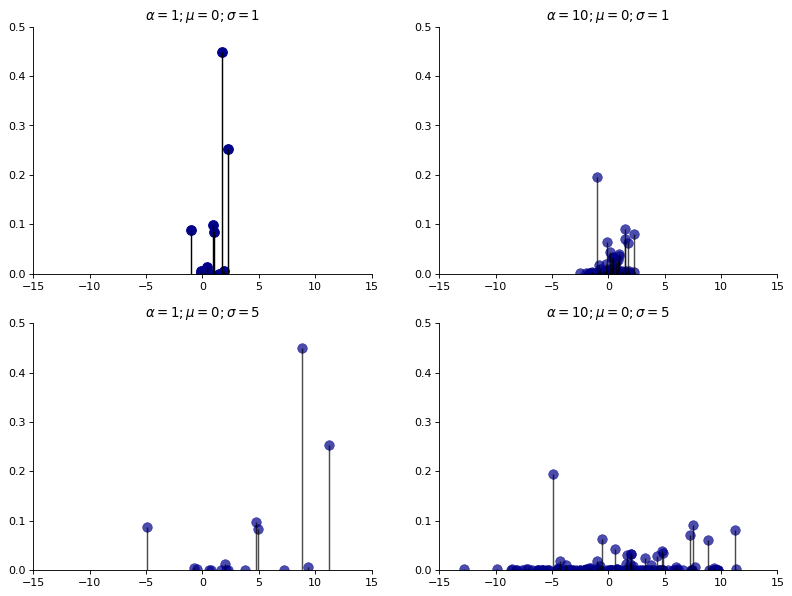
\includegraphics[scale=0.4]{dirichlet_process.png}
\caption{Random measure sampled from a Dirichlet Process with normal base measure. Height is proportional to mixture components.}
\end{figure}


\end{document}